
\documentclass[aspectratio=169]{beamer}
\usetheme{metropolis}           % Use metropolis theme
\usepackage[utf8]{inputenc}
\usepackage{graphicx}
\usepackage{eso-pic}
\usepackage{graphics}
\usepackage{tikz}
\usepackage[export]{adjustbox}
\usepackage{multicol}
\usepackage{listings}
\usepackage{helvet}
\usepackage{booktabs}
\usepackage{threeparttable}
\usepackage{fontspec}


\title{Topic 2 - Track 1 \newline Coding for Reproducible Research}
\date{\today}
\author{Meyhar Mohammed, Kristoffer Bjarkefur} % Name of author(s) of session here
\institute{Development Impact Evaluation (DIME) \newline The World Bank }
\setbeamercolor{background canvas}{bg=white}	% Sets background color

% The below command places the World Bank logo and DIME logo to the right corner
\titlegraphic{%
	\begin{picture}(0,0)
	\put(330,-180){\makebox(0,0)[rt]{
\includegraphics[width=3cm]{../../img/WB_logo}}}
	\end{picture}%
	\begin{picture}(0,0)
	\put(390,-180){\makebox(0,0)[rt]{
\includegraphics[width=1.5cm]{../../img/i2i}}}
	\end{picture}%
}

%%% Section page with picture of Light bulb
\makeatletter
\defbeamertemplate*{section page}{mytheme}[1][]{
	\centering
	\begin{minipage}{22em}
		\raggedright
		\usebeamercolor[fg]{section title}
		\usebeamerfont{section title}
		\par
		\ifx\insertsubsectionhead\@empty\else%
		\usebeamercolor[fg]{subsection title}%
		\usebeamerfont{subsection title}%
		\fi
		\ifstrempty{#1}{}{%
			\includegraphics[width=100mm, height=60mm]{#1}%
		}
		\insertsectionhead\\[-1ex]
		\insertsubsectionhead
		\usebeamertemplate*{progress bar in section page}

	\end{minipage}
	\par
	\vspace{\baselineskip}
}
\makeatother

%%% Define a command to include picture in section,
%%% make section, and revert to old template
\newcommand{\sectionpic}[2]{
	\setbeamertemplate{section page}[mytheme][#2]
	\section{#1}
	\setbeamertemplate{section page}[mytheme]
}

\usepackage{fancyvrb} % Allows customization of verbatim environments
%Fancyvrb docs: http://mirrors.ibiblio.org/CTAN/macros/latex/contrib/fancyvrb/doc/fancyvrb-doc.pdf
\fvset{fontsize=\scriptsize} % The font size of all verbatim text can be changed here

%So we can use option FloatBarrier, which is similar to [H] but is an
%alternative solition when the algorithm can't solce [H] as too many
%settings are going on. [H] seems to get stuck in infinite loop
%https://tex.stackexchange.com/questions/2275/keeping-tables-figures-close-to-where-they-are-mentioned
\usepackage{placeins}
\newcommand{\codeexample}[2]{
	\begin{figure}
		\VerbatimInput[
		framesep=3mm,
		frame=lines, % line above and below code section
		numbers=left, %Line number
		label= #1, %name of code section
		baselinestretch=0.90, %Use line space more similat to line space in code editors
		]{#2} %Write the relative file path and the name of the file to be included
	\end{figure}
	\FloatBarrier
}

\newcommand{\tinycodeexample}[2]{
	\begin{figure}
		\VerbatimInput[
		fontsize=\tiny,
		framesep=3mm,
		frame=lines, % line above and below code section
		numbers=left, %Line number
		label= #1, %name of code section
		baselinestretch=0.90, %Use line space more similat to line space in code editors
		]{#2} %Write the relative file path and the name of the file to be included
	\end{figure}
	\FloatBarrier
}


%% The below command creates the ligh bulb logos in the top right corner of the
\begin{document}

{
	\usebackgroundtemplate{
\includegraphics[height=55mm, right]{../../img/top_right_corner.pdf}}
	\maketitle
}

%%%%%%%%%%%%%%%%%%%%%%%%%%%%%%%%%%%%%%%%%%% heading of section 1
\sectionpic{Excel vs. Stata}{../../img/section_slide}


\begin{frame}{Why do we use Stata?}
\begin{center}
	\huge Can I use Excel?
\end{center}

\end{frame}


\begin{frame}{What's the fuss about do-files?}

\begin{itemize}
	\item It’s through the do-file you communicate your work to other members in your team, both current and future

	\item Think of the do-files as instructions on how to get from raw data to final report

	\item Also, for a simple task you can enter commands manually, but for more complex tasks you need to write a recipe, or a list of instructions

\end{itemize}
\end{frame}

\begin{frame}{The main reason we use Stata (or R)}
\begin{itemize}

	\item In Excel you make changes \underline{directly to the data} and \underline{save new versions of the data set}

	\item In Stata you make changes \underline{to the instructions} on how to get from the raw data to the final analysis and save \underline{new versions of the instructions}
\end{itemize}
\end{frame}

%%%%%%%%%%%%%%%%%%%%%%%%%%%%%%%%%%%%%%%%%%%
\sectionpic{How to open up a data set in Stata}{../../img/section_slide}

\begin{frame}{}
	\begin{figure}
		\centering
		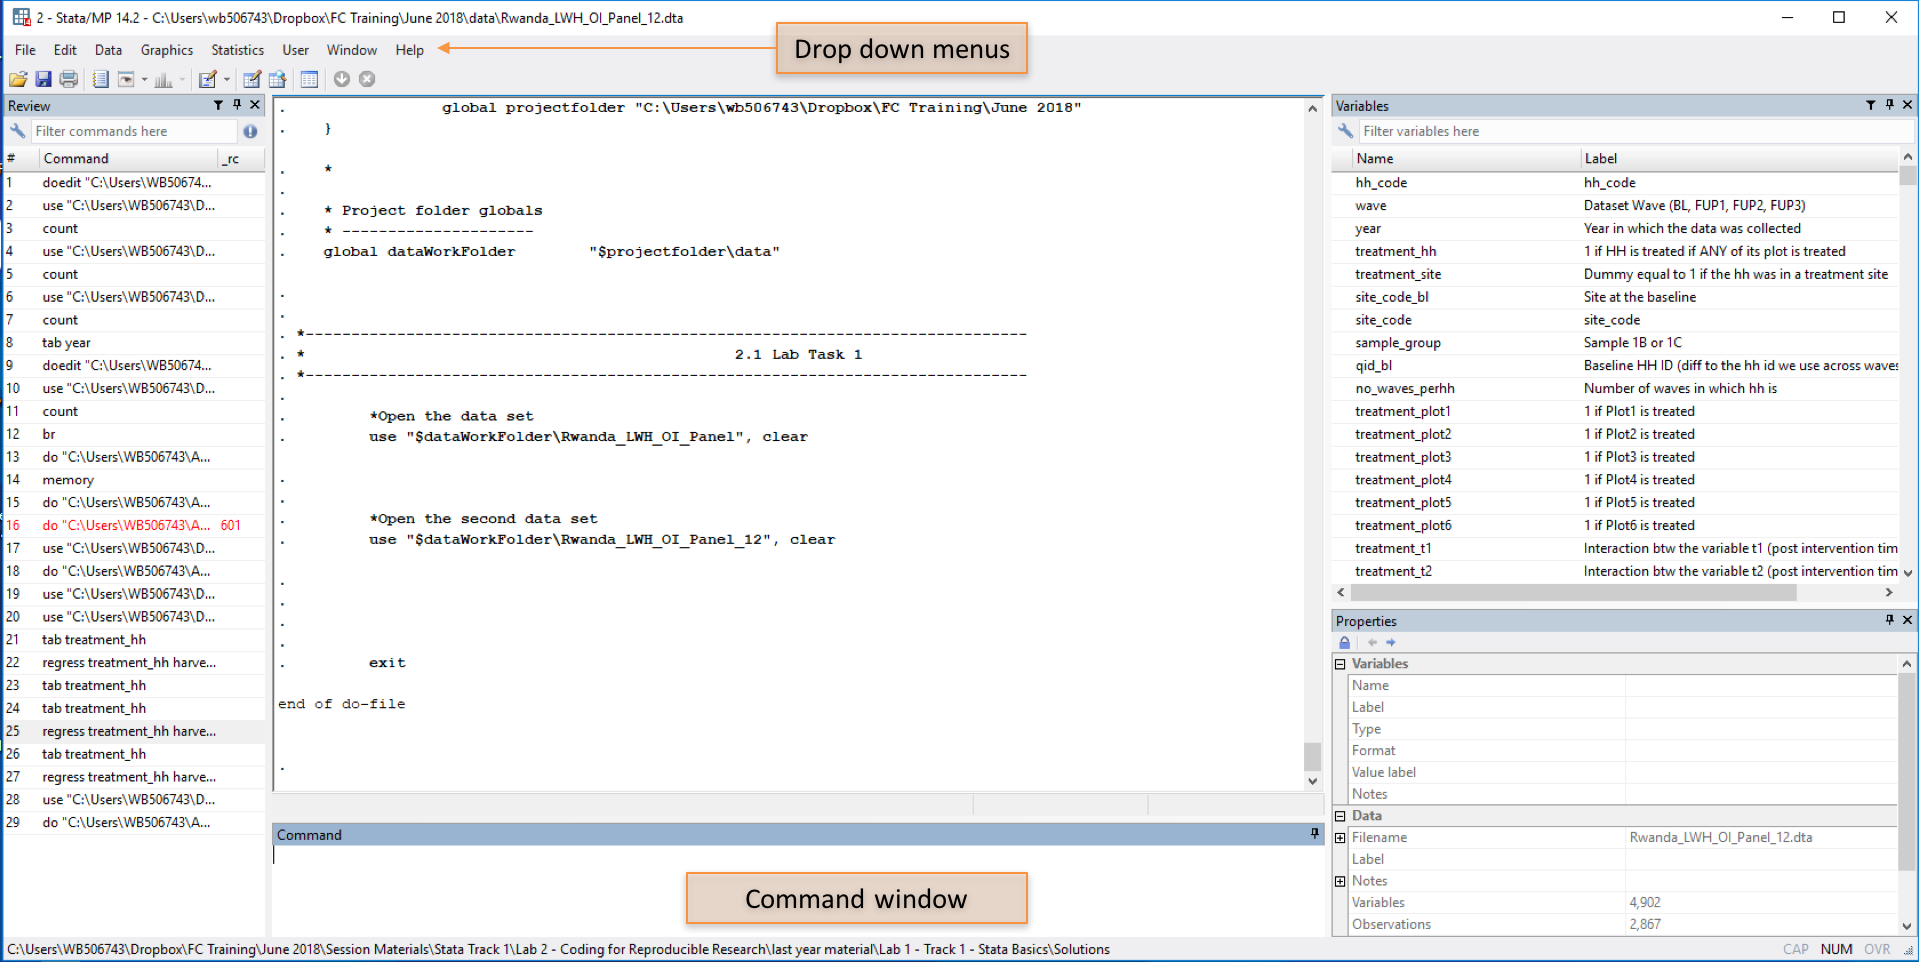
\includegraphics[width=\linewidth]{img/open_dataset}
	\end{figure}
\end{frame}

\begin{frame}{Three ways to tell Stata what to do}
	\begin{itemize}
		\item Drop-down menus
		\begin{itemize}
			\item An easy place to start but quickly becomes inefficient
		\end{itemize}
		\item Command window
		\begin{itemize}
			\item Faster than menus but require that you are familiar with the command
		\end{itemize}
		\item Do-file
		\begin{itemize}
			\item Use menus and command window to figure out what you need to write, then copy to a do file
			\item The only feasible way to run long instructions
		\end{itemize}
	\end{itemize}
\end{frame}

\begin{frame}{}
	\begin{figure}
		\centering
		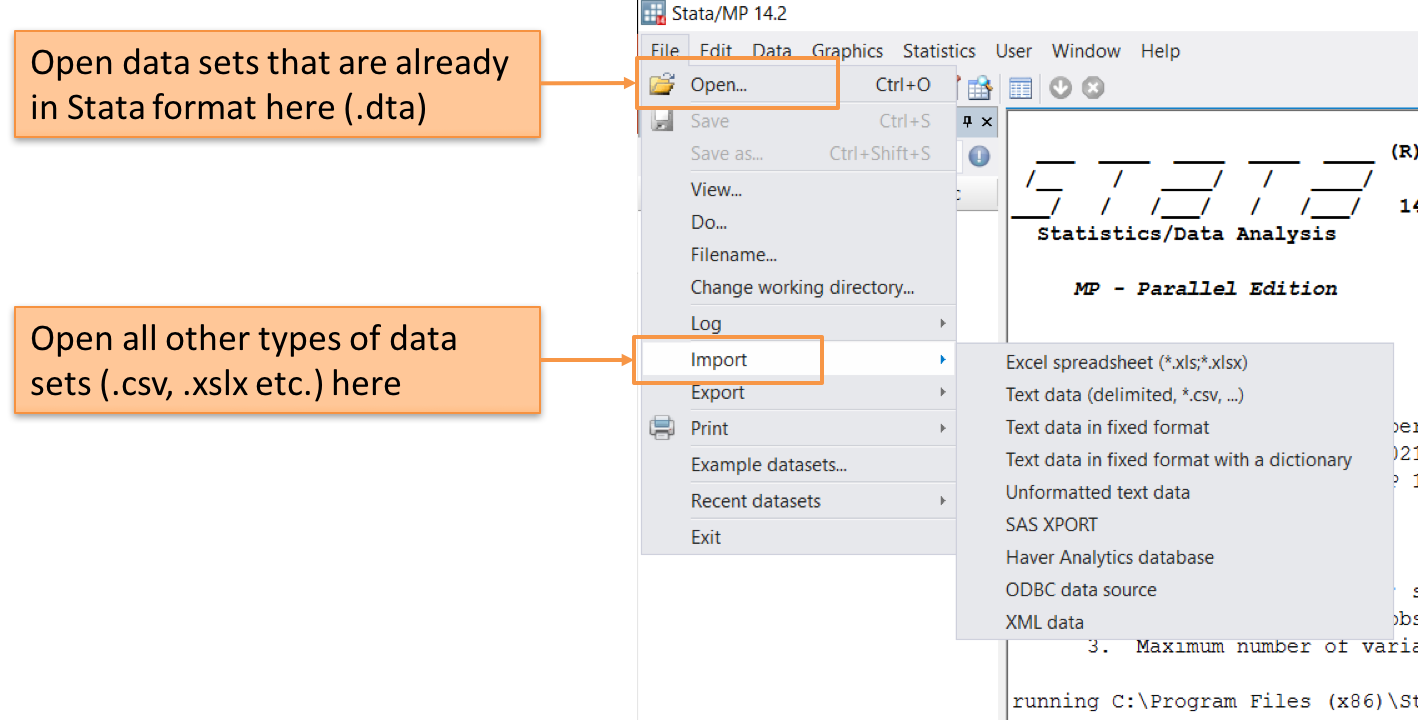
\includegraphics[width=\linewidth]{img/open_dataset_menu}
	\end{figure}
\end{frame}

\begin{frame}[fragile]{Open a dataset - command window}
	\begin{figure}
		\centering
		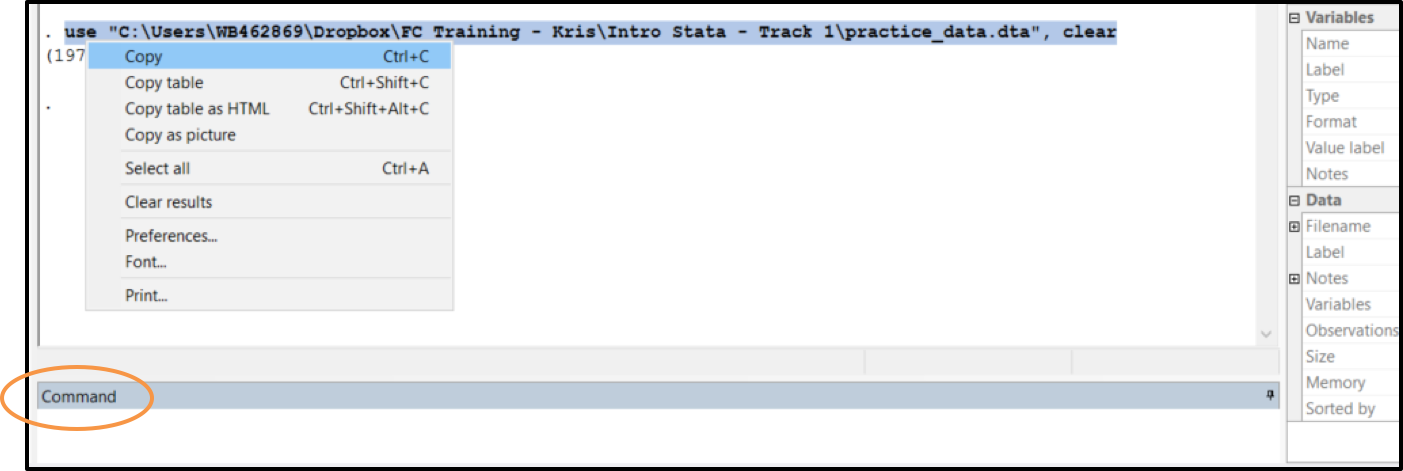
\includegraphics[width=\linewidth]{img/open_data_command}
	\end{figure}
	\begin{itemize}
		\item When you use the menus, Stata produces the code for that action
		\item Highlight, right-click and copy the code. Paste the code in the command window. And hit enter.
	\end{itemize}
\end{frame}

\begin{frame}{Task 1 - Open data}
	\begin{itemize}
		\item Open Stata and then open data set \texttt{endline\_data\_raw\_nodup.dta} using the menu: File -> Open. Navigate to where you saved the material for this lab. Select the data set and click Open.
		\item Browse to check that you have data: Data -> Data Editor -> Data Editor Browse
		\item Copy the code Stata generated for you and paste it in the command window. Hit enter and then browse the data again.
		\item Copy and paste the code again. But this time, change the code so that you open \texttt{panel\_data.dta} instead. You do not have to use the menus again, just change the filename in the line of code you just copied. Browse the data!
		\item We will introduce do-files very soon
	\end{itemize}
\end{frame}


%%%%%%%%%%%%%%%%%%%%%%%%%%%%%%%%%%%%%%%%%%%
\sectionpic{An introduction to Stata: Stata interface (what are all those windows)}{../../img/section_slide}

\begin{frame}{}
	\begin{figure}
		\centering
		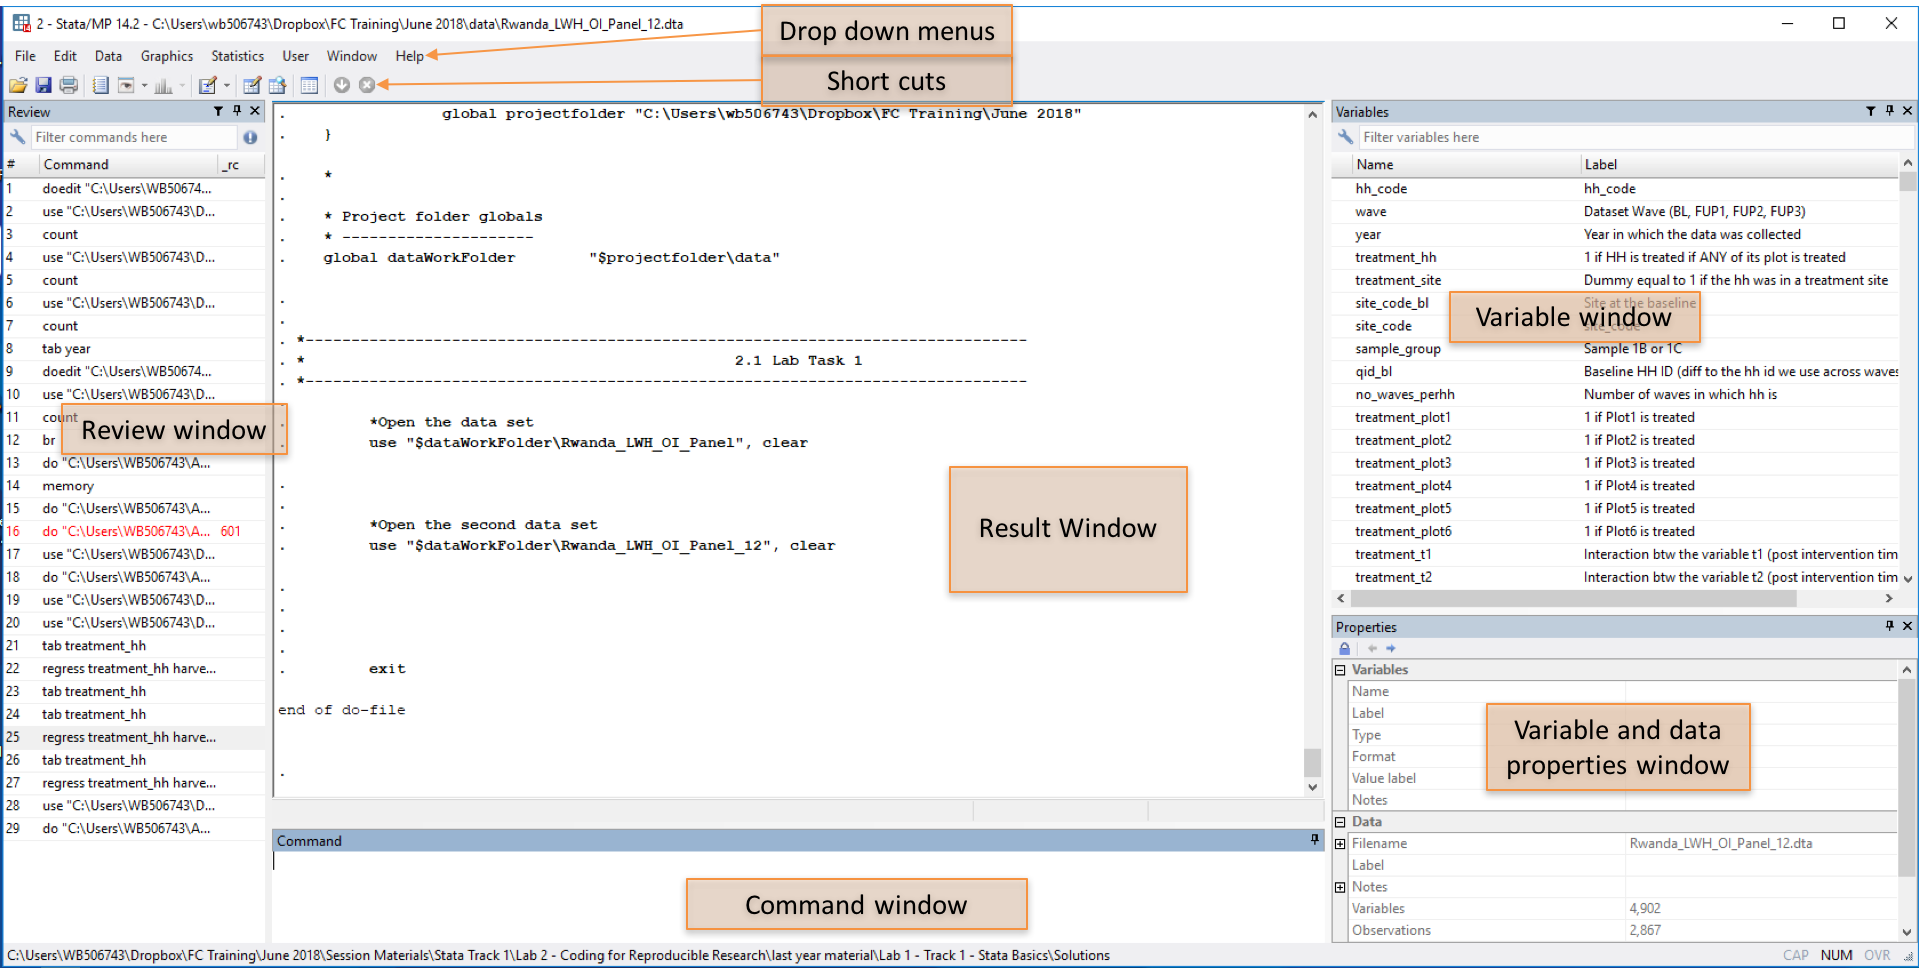
\includegraphics[width=\linewidth]{img/window_des}
	\end{figure}
\end{frame}

\begin{frame}{Review Window}

\begin{itemize}
	\item In the last task we asked you to copy and paste from the result window. That works, but the best practice way to do it is using the review window.

	\item Double click on a command you want to use again and it will appear in your command window
	\begin{itemize}
		\item You can also click in command window and select the commands in the result window by using PageUp/PageDown buttons
		\item fn+ArrowUp/ fn+ArrowDown on Mac
	\end{itemize}
	\item If a command is red in the review window, it means it hit an error and did not finish
\end{itemize}
\end{frame}

\begin{frame}[fragile]{Text and Image}
	\begin{columns}[c]
		\column{.6\textwidth}
		\begin{itemize}
			\item Both the variable window and the review will soon be very crowded. You can then search both of them
			\item If you do not see the search bar, click the little funnel symbol
		\end{itemize}

		\column{.4\textwidth}
		\begin{figure}
			\centering
			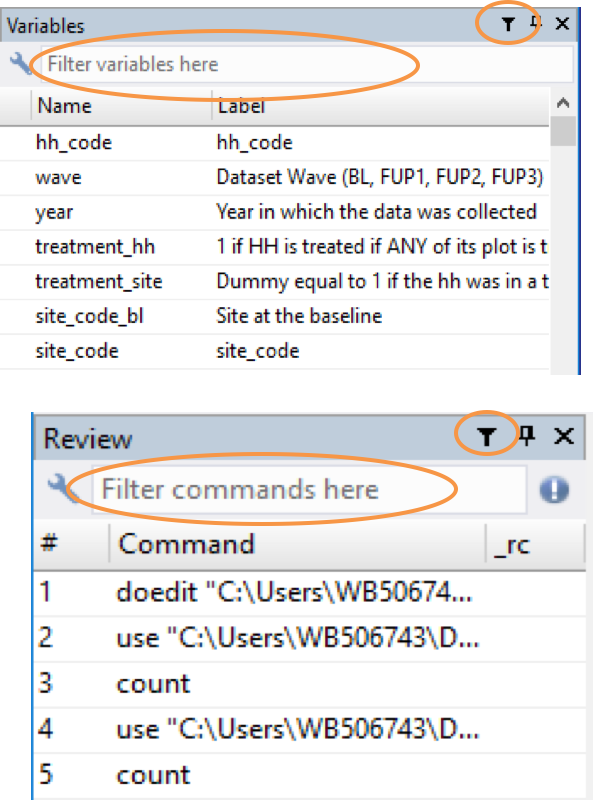
\includegraphics[width=.75\linewidth]{img/review_window}
		\end{figure}
	\end{columns}
\end{frame}

%%%%%%%%%%%%%%%%%%%%%%%%%%%%%%%%%%%%%%%%%%%

\sectionpic{An introduction to Stata: \newline Exploring a data set opened for the first time}{../../img/section_slide}


\begin{frame}{Exploring a new dataset}
	\begin{itemize}
		\item \texttt{browse}: see all data in spreadsheet format
		\item \texttt{describe}: list of all variables in memory
		\begin{itemize}
			\item Total number of variables \& observations (size of matrix)
			\item Variable name, type, format, value label name, variable label
		\end{itemize}
		\item \texttt{summarize}: Basic statistics for numeric variables
		\begin{itemize}
			\item N, mean, standard deviation, min, max
			\item \texttt{summarize, detail}: percentiles, variance, skewness, kurtosis
		\end{itemize}
		\item \texttt{tabulate}: frequencies
	\end{itemize}
\end{frame}


\begin{frame}{Types of variables}
\begin{itemize}
	\item In Stata, each variable (column) has to be either:
	\begin{itemize}
		\item string (text) – values are red when browsing.
		\item numeric (number) – values are black or blue when browsing
	\end{itemize}
	\item Numbers can be stored as text, but text cannot be stored as number.
	\begin{itemize}
		\item 	However, not possible to do computations on numbers stored as text
	\end{itemize}
	\item Categorical variables should be stored as numeric variables and have labels.
\end{itemize}
\end{frame}

\begin{frame}{Task 2 - Explore the data}
	\begin{itemize}
		\item Open \texttt{endline\_data\_raw\_nodup.dta} again.
		\item Which variables are string and which are numeric?
		\begin{itemize}
			\item \texttt{browse} – see the different colors in the columns.
			\item \texttt{describe} – see the column storage type.
			\item \texttt{summarize} – why is there no mean for some variables, for example \texttt{comment}?
		\end{itemize}
		\item Learn more about the variable \texttt{numplots}. What values does it take on? What is minimum? Maximum? Mean? How many unique values?
		\begin{itemize}
			\item \texttt{tabulate numplots}
			\item \texttt{summarize numplots} or \texttt{summarize numplots, detail}
			\item \texttt{codebook numplots}
		\end{itemize}
	\end{itemize}
\end{frame}

\sectionpic{An introduction to Stata: - Generating new variables and labeling them}{../../img/section_slide}

\begin{frame}[fragile]{Create new variables}

	\begin{itemize}
		\item \texttt{generate} a variable with the household income by household size
		\item \texttt{generate} a dummy variable that is 1 if per capita of income is more than 10,000 KG.
	\end{itemize}

	\codeexample{generate.do}{code/generate.do}

\end{frame}

\begin{frame}[fragile]{Label variables you create}
\begin{itemize}
	\item You will thank yourself if you carefully document what you do. You will not remember everything a month later.
	\item Label all variables you create, so that future you and others understand.
\end{itemize}
	\vspace{.5cm}
	\codeexample{variable-labels.do}{code/variable-labels.do}
\end{frame}

\begin{frame}[fragile]{Value labels}
	\begin{itemize}
		\item For all categorical variables, you should also create value labels, to indicate what each category stand for.
		\item In the example below we apply a label explaining the dummy we just created. This variable will now be very clear to anyone using this data set.
	\end{itemize}
	\vspace{.5cm}
	\codeexample{value-labels.do}{code/value-labels.do}
\end{frame}

\begin{frame}{Lab Task 3}
	\begin{itemize}
		\item The variable \texttt{inc\_01} indicates the household income from on-farm enterprise in Rwanda Francs. Create a new variable that depicts it in US dollars. About 0.0012 USD exchanges to 1 Rwanda franc. Call the new variable \texttt{inc\_01\_USD}. And label it appropriately.
	\end{itemize}
	\codeexample{task-3.do}{code/task-3.do}
	\begin{itemize}
		\item Use the same code and create the variable \texttt{inc\_01\_EUR0}. (1 RWF= .0001 Euro.) Remember to also label it!
		\item Create a dummy variable for high on-farm enterprise income in the same way \texttt{high\_income} was created. Use the cut-off 5,000  Euros. Remember to label it!
	\end{itemize}
\end{frame}

%%%%%%%%%%%%%%%%%%%%%%%%%%%%%%%%%%%%%%%%%%%
\sectionpic{An introduction to Stata: \newline How to share your work with your team}{../../img/section_slide}

\begin{frame}{You are asked to share your work}
	\begin{itemize}
		\item How would you share the work you have done so far?
		\item Send only the data set? That would be like Excel and only share the latest version of the data.
		\item In research we need to share more than the latest version of the data. We need to show what we did.
		\item Yes, you guessed it, it is time to introduce the do-file.
	\end{itemize}
\end{frame}

\begin{frame}{Do-files}
	\begin{itemize}
		\item Open up a new do-file. Window -> Do-file Editor -> New Do-file Editor. Or click the shortcut highlighted below:
		\begin{figure}
			\centering
			
\includegraphics[width=.6\linewidth]{img/dofilewindow1}
		\end{figure}
		\item Treat the do-file similarly to how you treat the command window. But instead of copying and running one line of code at the time, a do-file lets you do that with any number of lines of code.
		\item Running the code in your do-file using menus: Tools -> Execute (Do). Or Ctrl+D (Windows) or this short cut:
		\begin{figure}
			\centering
			
\includegraphics[width=.5\linewidth]{img/dofilewindow2}
		\end{figure}
	\end{itemize}
\end{frame}

\begin{frame}{Task 4 - Do-files}
	\begin{itemize}
		\item Open a new do-file. Save it! Go to the review window and copy the code where you loaded \texttt{endline\_data\_raw\_nodup.dta}. Now run your do-file.
		\item Next, use the review window to copy to your do-file all the actions you already did:
		\begin{itemize}
			\item Open data \texttt{endline\_data\_raw\_nodup.dta} (done in Task 1 above)
			\item Explore the data
			\item Generate \texttt{inc\_per\_hh\_member} and \texttt{inc\_01\_USD}
			\item Label \texttt{inc\_per\_hh\_member} and \texttt{inc\_01\_USD}
			\item Create and label the \texttt{high\_income} variable
			\item Now run your do-file again. You have written instructions how to get to the \texttt{endline\_data\_raw\_nodup.dta} to the final version
		\end{itemize}
	\end{itemize}
\end{frame}

\begin{frame}{Comments}
	\begin{itemize}
		\item Comments is the green text you have seen in the code examples. Comments is text that Stata will ignore when running your code.
		\item Comments is what makes the difference between instructions that are easy to follow or impossible to understand.
	\end{itemize}
\end{frame}

\begin{frame}{Different types of comments}
	\begin{itemize}
		\item \texttt{/* ...comment... */} -> Used for long comments or to explain many lines of code in the following section
		\item \texttt{* ...comment...} -> Used to explain what happens on the following few rows
		\item \texttt{// ...comment...} -> Used to explain the same line of code
	\end{itemize}
\end{frame}

\begin{frame}{Task 5}
	\begin{itemize}
		\item Comment your code! It is really important to get into a habit of commenting code really well if you want to become a really good programmer!
		\item Comment your code so far as much as possible, but make sure to use each comment type at least once:
	\end{itemize}
	\begin{itemize}
		\item \texttt{/* ...comment... */}
		\item \texttt{* ...comment...}
		\item \texttt{// ...comment...}
	\end{itemize}
\end{frame}

%%%%%%%%%%%%%%%%%%%%%%%%%%%%%%%%%%%%%%%%%%%

\sectionpic{Other features of Stata: - Using macros (globals, locals and scalars)}{../../img/section_slide}

\begin{frame}{Macros}
	\begin{itemize}
		\item You need to be at least familiar with this topic for the resources you will be introduced to this week.
		\item This technique is critical as projects grow in size. But even the smallest DIME project absolutely needs this.
		\item Macros (globals, locals, scalar) save some information (text or number) that you can reference later.
			\begin{itemize}
				\item Example, we want to access files in the folder multiple times. We can store the folder location in a global and use it multiple times.
			\end{itemize}
	\end{itemize}
\end{frame}

\begin{frame}{Defining macros - locals}
	When running the code this becomes: \texttt{generate result\_var = (3 * 5) – 3}
	\codeexample{macros-local.do}{code/macros-local.do}
\end{frame}

\begin{frame}{Defining macros - globals}
	This create two variables:
	\begin{itemize}
		\item One variable that is called \texttt{country\_GAFSP} and with the value Kenya for all observations.
		\item One variable that is called \texttt{donor\_GAFSP} with the value World Bank for all observations.
	\end{itemize}
	\codeexample{macros-global.do}{code/macros-global.do}
\end{frame}

\begin{frame}{Setting directories using macros}

	\tinycodeexample{filepaths-1.do}{code/filepaths-1.do}

	\small The code above and below is the same to Stata. But the part that is the identical in use and save is stored in and referenced from a global below, and the line of code is shorter and more readable
	\codeexample{filepaths-2.do}{code/filepaths-2.do}
\end{frame}

\begin{frame}{Lab Task 6}
	\begin{itemize}
		\item Open the do-file you created in the previous task and create a global to the folder where you have been saving your work. Call the global \texttt{folder\_Lab1}
		\item To check what is stored in your global, type this in the command window and hit enter:
			\begin{itemize}
				\item \texttt{display "\$\string{folder\_Lab1\string}“}
			\end{itemize}
		\item Update the use and save commands in your do-file with the global you created. See example blow. Then re-run your code to make sure that it works with the new file paths!
	\end{itemize}
	\codeexample{filepath-example.do}{code/filepath-example.do}
\end{frame}


%%%%%%%%%%%%%%%%%%%%%%%%%%%%%%%%%%%%%%%%%%%
\sectionpic{Other Features of Stata: \newline White Space}{../../img/section_slide}

\begin{frame}[t]{.}
	\begin{columns}[t]
		\column{.7\linewidth}
		\begin{figure}
			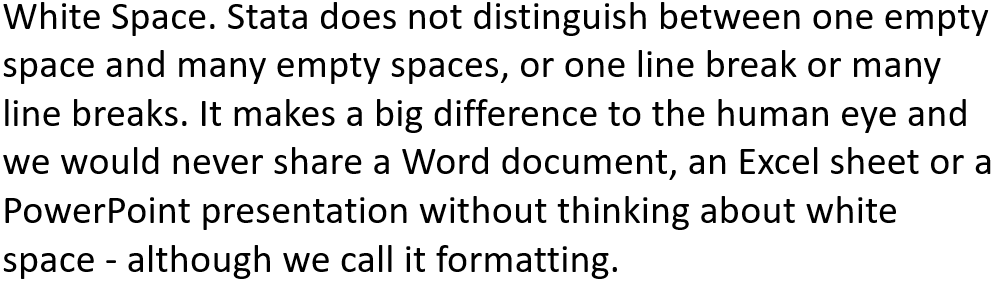
\includegraphics[width=\linewidth]{img/white-space}
		\end{figure}
		\column{.3	\linewidth}
	\end{columns}
\end{frame}


\begin{frame}{White Space}
	\begin{itemize}
		\item Stata does not distinguish between one empty space and many empty spaces, or one line break or many line breaks
		\item It makes a big difference to the human eye and we would never share a Word document, an Excel sheet or a PowerPoint presentation without thinking about white space – although we call it formatting
	\end{itemize}
\end{frame}

\begin{frame}{White Space - columns}	
	\codeexample{white-space-columns.do}{code/white-space-columns.do}
\end{frame}



%%%%%%%%%%%%%%%%%%%%%%%%%%%%%%%%%%%%%%%%%%%
\sectionpic{Other Features of Stata: \newline Missing values}{../../img/section_slide}

\begin{frame}{Missing Values}
	\begin{itemize}
		\item String variables can be empty, but numeric variables can’t be empty. Instead numeric variables have something called “missing values”.
			\begin{itemize}
				\item 	Missing values are represented in Stata with a dot, like this: \texttt{.}
				\item You can also use \texttt{.a} or \texttt{.b} etc. to \texttt{.z} for missing values and you will learn later how these can be used.
			\end{itemize}
		\item Stata can’t use missing values in computations (averages, regressions etc.) so it skips observations with missing values.
		\item Missing values changes the analysis as observations with missing values are excluded from commands like summarize and regress.
		\item Good practice to always check for missing values when tabulating variables.
	\end{itemize}
\end{frame}

\begin{frame}{Lab Task 7 - Missing values}
	\begin{itemize}
		\item Make sure that you have the \texttt{endline\_data\_raw\_nodup.dta} with the edits you already made open.
		\begin{itemize}
			\item Type \texttt{summarize inc\_*} into the command window. Look at the column obs in the output. What do you notice?
			\item There are  1,064 observations in the data set, but less than 1,064 observations were included in the output for the income variables. Why is that?
		\end{itemize}
		\item \texttt{misstable summarize} identifies and reports missing values in all the variables in your data set. Use the command on the income variables - \texttt{misstable summarize inc\_*} and see that it reports exactly 105 missing observations for the main household income variables. That explains why we had less than 1,064 observations.
		\item Another way to investigate the missing observations is to tabulate variable \texttt{inc\_zero}.
		\begin{itemize}
			\item Test first: \texttt{tabulate inc\_zero}, then test: \texttt{tabulate inc\_zero, missing}
		\end{itemize}
	\end{itemize}
\end{frame}

\sectionpic{An introduction to Stata: \newline Saving your datasets}{../../img/section_slide}

\begin{frame}{Lab Task 8 - Saving Stata datasets}
	\begin{itemize}
		\item Use the drop down menu to save your data under a different name, for example \texttt{endline\_data\_post\_topic2.dta}. File -> Save as. If you use Save instead of Save as you will not be asked to save under a new name
		\item Copy the code generated when using the menu to your do-file. Run again. Did you get an error?
			\begin{itemize}
				\item Since you already saved the data set under the new name, Stata warns you that there already is a file with that name. We want to overwrite it as each time we make an update to the instructions, we want the final data to reflect that. We therefore need to add a comma and the word replace.
				\item \texttt{save "\$\{folder\_Lab1\}/endline\_data\_post\_topic2.dta", replace}
			\end{itemize}
		\item Run your code again. Now you both have a final version of your data set and the instructions on how to get there. When your supervisor wants to see your work, share both of these!
	\end{itemize}
\end{frame}


\sectionpic{Other features of Stata: \newline Open non-Stata data sets}{../../img/section_slide}

\begin{frame}[fragile]{Importing data from .xls/.xslx or .csv}
	\begin{columns}[c]

		\column{.5\textwidth}
		\begin{itemize}
			\item Always start by using the drop down menus if you do not know the command!
			\item Select the format of your file:
			\begin{itemize}
				\item Excel (.xls,.xlsx)
				\item plain text delimited (.txt)
				\item comma separated (.csv)
			\end{itemize}
			\item Select the appropriate choice in the menu and follow the instructions.
			\item Copy the code Stata Generates for you and put it in your do-file.
		\end{itemize}

		\column{.5\textwidth}
		\begin{figure}
			\centering
			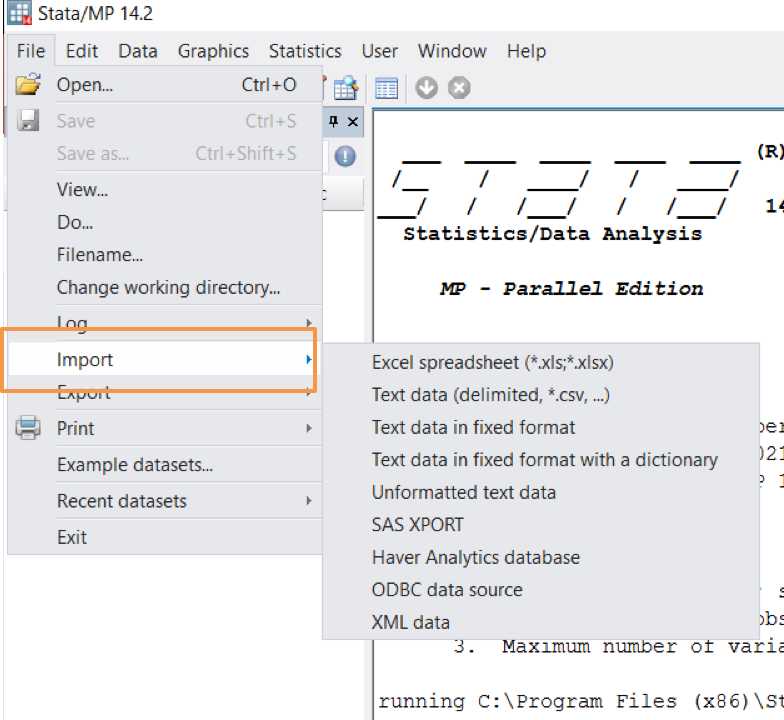
\includegraphics[width=\linewidth]{img/importcsv}
		\end{figure}
	\end{columns}
\end{frame}

\begin{frame}{Lab Task 9 - Import other types of data}
	\begin{itemize}
		\item \small Use the drop down menus to import the \texttt{village\_codes.xls} data to Stata. Use all default options for now, so click \texttt{OK} for everything.
		\begin{itemize}
			\item \small Use \texttt{describe}, \texttt{tabulate}, \texttt{browse} or any other tools you have learned to explore the data. What are your key observations?
		\end{itemize}
		\item \small In Excel the first row can be used as variable names, but in Stata the first row is always data. Use the drop-down menu to import that data again, but see if you find an option that solves this before clikcing \texttt{OK}. Use the option you think is suitable for this, and explore the data again. What is different?
		\item \small In the result window or in the review window, see that the two lines of code generated are similar, but have the difference that the second time the word \texttt{firstrow} is used at the end. Include this option when you copy your code to your do-file.
		\item \small It is a very good practice to use the drop down menus and the command window to experiment with your code until you are happy with it. When you are happy with the code Stata generates to import \texttt{village\_code.xls}, copy that line of code to your do-file and use the global you created in Task 6 to shorten the file path
	\end{itemize}
\end{frame}

%%%%%%%%%%%%%%%%%%%%%%%%%%%%%%%%%%%%%%%%%%% Final thougts section
\begin{frame}{Conclusion}


\vspace{20mm}
For more information or further questions please contact:
\newline Kristoffer Bjarkefur (\url{kbjarkefur@worldbank.org}) \newline Mary Doe (\url{marydoe@worldbank.org})

\end{frame}

%%%%%%%%%%%%%%%%%%%%%%%%%%%%%%%%%%%%%%%%%%% The End
\sectionpic{Thank You!}{../../img/section_slide}

\end{document}
